% Theorem environments
\newtheorem{definition}{Definition}
\newtheorem{theorem}{Theorem}
\newtheorem{example}{Example}
\newtheorem{lemma}{Lemma}

\newtheorem{cor}{Corollary}
\newtheorem{prop}{Proposition}
\newtheorem{rem}{Remark}

\def\N{{\mathbb N}} 
\def\E{{\rm E}} 
\def\P{{\rm P}} 

\def\sign{{\rm sign}}

\def\sp{{\sigma_{\rm p}}}
\def\ia{\Delta I}
\def\ha{\Delta H}
\def\ip{\Delta_{\rm p}I}
\def\hp{\Delta_{\rm p} H}
\def\simp{s_{\rm p}}
\def\qp{q_{\rm p}}

\def\be{\begin{equation}}
\def\ee{\end{equation}}
\def\bp{\noindent {\it Proof.}\ }
\def\ep{\hfill $\Box$} 

\chapter{Methodology}
\label{design}

This Chapter presents a novel Information Theoretic Metric for Labeled Trees named Tree Mutual Information(TMI), which can be interpreted through the mutual information score and its expected value. The metric is based on a maximum alignment between leaves sets in labeled trees. We first explain the relation of our novel metric to information theory, show the application of adjusted mutual information in this context, and introduce a novel adjustment based on pairwise label permutations instead of full label permutations. We show that the corresponding adjusted metric can be expressed explicitly and behaves similarly to the standard adjusted mutual information for assessing the quality of clustering while having a much lower time complexity. Both metrics are adopted to be used as a construction element of a tree comparison solution.

Most of the proofs in this Chapter can be found in our publication \cite{Lazarenko2021pairwise}. 

\section{Information Theory}
Let $P$ be the uniform probability measure on  $\Omega = \{1,\ldots,n\}$, for some positive integer $n$. Let $X,Y$ be random variables on the probability space $(\Omega, P)$. Without any loss of generality, we assume that  $X$ and $Y$ are mapping from $\Omega$ to sets consisting of  consecutive integers, starting from 1.
Denoting by $H$ the entropy, the mutual information between $X$ and $Y$ is defined by \cite{cover}:
\be\label{eq:info}
I(X, Y) = H(X) + H(Y) - H(X,Y).
\ee
This is the information shared by $X$ and $Y$, which is equal to 0 if $X$ and $Y$ are independent.
A distance between $X$ and $Y$ can then be defined by:
$$%\be\label{eq:d}
d(X,Y) = H(X,Y) - I(X,Y) = H(X|Y) + H(Y| X).
$$%\ee
This distance, known as the variation of information, is a metric in the quotient space of random variables under the equivalence relation $X\sim Y$ if and only if there is some bijection $\varphi$ such that $X = \varphi(Y)$ \cite{vi}.

\paragraph{Adjusted mutual information.}
The adjusted mutual information between $X$ and $Y$, corresponding to  the mutual information between $X$ and $Y$ {\it adjusted} against chance, is defined by:
\be\label{eq:def}
\ia(X,Y) = I(X,Y) - \E(I(X, Y_\sigma)),
\ee
where  $Y_\sigma$ is the random variable $Y \circ \sigma$, for any   permutation $\sigma$ of $\{1,\ldots, n\}$, and the expectation is taken over all permutations $\sigma$, chosen uniformly at random. 

\begin{rem}[Normalization]\label{rem:norm}
	It is also frequent to normalize adjusted mutual information to get a score between 0 and 1 \cite{vinh2010information,romano2014standardized}. In this work, we only focus on the adjustment step. 
\end{rem}

Definition:
\begin{align}
\ia(X,Y) &=\E(H(X, Y_\sigma)) - H(X,Y),\nonumber \\ 
&= \frac 1 2 (\E(d(X, Y_\sigma)) - d(X,Y)).\label{eq:dist}
\end{align}
This equivalence follows from Proposition 1 and the fact that the definition is symmetric
in X and Y. All proofs could be found in the \cite{Lazarenko2021pairwise}.

\begin{prop}\label{prop:equiv}
	We have for any random variables $X$ and $Y$:
	\begin{align*}
	H(X)&= \E(H(X_\sigma)),\\
	\E(H(X, Y_\sigma)) &= \E(H(X_\sigma, Y)),\\
	\E(I(X, Y_\sigma)) &= \E(I(X_\sigma, Y)).
	\end{align*}
\end{prop}

In view of \eqref{eq:dist}, we expect $\ia(X,Y)$ to be positive if $X$ and $Y$ share information, as $X$ is expected to be closer to $Y$ (for the distance $d$)  than to $Y_\sigma$, a randomized version of $Y$. 
There are specific cases where $\ia(X,Y)=0$, as stated in 

\begin{prop}\label{prop:zero}
	We have $\ia(X,Y)=0$  whenever $Y$ (or $X$, by symmetry) is constant or equal to some permutation of  $\{1,\ldots,n\}$.
\end{prop}

\paragraph{Adjusted entropy.} Observing that $H(X) = I(X, X)$, 
we define similarly the adjusted entropy of $X$ by:
$$
\ha(X) = \ia(X,X) =  H(X) - \E(I(X, X_\sigma)).
$$
By \eqref{eq:info}, we get:
\be\label{eq:ae2}
\ha(X) =\E(H(X, X_\sigma)) - H(X)= \frac 12 \E(d(X,X_\sigma)).
\ee
Since $d$ is a metric, this shows that the adjusted entropy of $X$ is non-negative. 

\begin{prop}\label{prop:entropy}
	We have $\ha(X) = 0$ if and only if  $X$ is constant or equal to some permutation of $\{1,\ldots,n\}$.
\end{prop}

Proposition \ref{prop:entropy} characterizes random variables with zero adjusted entropy. 
Proposition results will be interpreted in terms of clustering in section \ref{sec:cluster}.

\section{Pairwise adjustment}

In this section, pairwise adjusted mutual information is introduced. 
The definition is the same as adjusted mutual information, except that  the permutation  $\sigma$ is now restricted to the 
set of pairwise permutations. Specifically, we consider permutations $\sigma$ for which there exists $i,j \in \{1,\ldots,n\}$ 
such that $\sigma(i) = j$ and $\sigma(j) = i$, whereas $\sigma(t) = t$ for all $t\ne i,j$.
We consider the set of such permutations $\sigma$ where the samples $i,j$ are drawn uniformly at random in the 
set $\{1,\ldots,n\}$. We denote by $\sp$ such a random permutation. Observe that $\sp$ is the identity with probability 
$1/n$ (the probability that $i=j$). 

\paragraph{Pairwise adjusted mutual information.}
We  define the {\it pairwise adjusted mutual information} as:
$$
\ip(X,Y) = I(X,Y) - \E(I(X, Y_\sp)).
$$
This is exactly the same definition as the adjusted mutual information, except for the considered permutations $\sp$. 
It can be readily verified that the same properties apply, with the exact same proofs, a key property being that the 
random permutations $\sp$ and $\sp^{-1}$ have the same distributions.

In particular, we  have the analogue of \eqref{eq:dist}:
\begin{align}
\ip(X,Y)& =\E(H(X, Y_\sp)) - H(X,Y),\nonumber\\
&= \frac 1 2 (\E(d(X, Y_\sp)) - d(X,Y)). \label{eq:ip2} 
\end{align}
Moreover, $\ip(X,Y)=0$ whenever $X$ or $Y$ is 
constant or equal to some permutation of $\{1,\ldots,n\}$.

\paragraph{Pairwise adjusted entropy.}
We  also define the {\it pairwise adjusted entropy} as:
$$
\hp(X) = \ip(X,X) =  H(X) - \E(I(X, X_\sp)).
$$
We have $\hp(X) \ge 0$, with equality if and only if  $X$ is constant or equal to some permutation of $\{1,\ldots,n\}$.


\section{Data processing inequality}
The following results give two versions of the data processing inequality for the adjusted mutual information.  We write $X\prec Y$ if $X = f(Y)$ for some mapping $f$. The proofs are deferred to the Appendix.

\begin{theorem}\label{th:ineq}
	If $X\prec Y$, then 
	$$ 
	\ia(X, Y) \le \ia(X,X).$$
	Moreover, the inequality is strict whenever $0 < H(X) < H(Y)$.
\end{theorem}

\paragraph{Proof of Theorem \ref{th:ineq}.}
Since $X \prec Y$,  
we have  $H(X|Y) = 0$ and
$$
I(X,Y) = H(X) - H(X|Y) = H(X) = I(X,X).
$$
Now for any permutation $\sigma$ of $\{1,\ldots,n\}$, we have $I(X_\sigma, Y) \ge I(X_\sigma, X)$ by the data processing inequality \cite{cover}, 
which implies:
$$
\ia(X, Y) \le  \ia (X, X).
$$

Now assume that $0 < H(X) < H(Y)$.
To prove that the inequality is strict, let $\sigma$ be the permutation of  $a, b \in\{1,\ldots,n\}$ with $X(a) \ne X(b)$.  Let $i  = X(a), j= X(b)$ and $A = \{\omega: X(\omega) = i\}, B=\{\omega: X(\omega) = j\}$. 
We get:
$$
\P(X_\sigma=j | X=i) =  \frac 1 {|A|},\quad  \P(X_\sigma=i | X=j) =  \frac 1 {|B|}, \quad 
\P(X_\sigma=k | X=k) =  1\quad \forall k\ne i, j,
$$
so that:
$$
H(X_\sigma |X)= \frac{|A|}n  H\left( \frac 1 {|A|}\right) + \frac{|B|}n  H\left( \frac 1 {|B|}\right),
$$
with $H(p) = -p\log p - (1-p)\log(1-p)$ the entropy of a Bernoulli random variable with parameter $p$.

Now let $i' = Y(a), j'= Y(b)$ and $A' = \{\omega: Y(\omega) = i\}, B'=\{\omega: Y(\omega) = b\}$. Observe that $i = f(i')$ and $j = f(j')$,  where $f$ is the mapping such that $X = f(Y)$, so that $i' \ne j'$. Moreover, $|A'| \le |A|$ and $|B'|\le |B|$. Since $H(Y) > H(X)$, we can choose $\sigma$ such that $|A'|< |A|$ or $|B'|<|B|$. We have:
$$
\Pr(X_\sigma=j | Y=i') =  \frac 1 {|A'|},\quad  \Pr(X_\sigma=i | Y=j') =  \frac 1 {|B'|}, \quad 
\Pr(X_\sigma=f(k) | Y=k) =  1
$$
so that:
$$
H(X_\sigma |Y)= \frac{|A'|}n  H\left( \frac 1 {|A'|}\right) + \frac{|B'|}n  H\left( \frac 1 {|B'|}\right).
$$

Since the mapping $t \mapsto t H\left(\frac 1 t\right)$ is  increasing over $(1,+\infty)$, we get:
$$
H(X_\sigma |Y) < H(X_\sigma |X)
$$
and
$$
I(X_\sigma,Y) = H(X_\sigma) -  H(X_\sigma |Y) > H(X_\sigma) -  H(X_\sigma |X) =   I(X_\sigma,X).
$$
In particular, $\E(I(X_\sigma, Y)) > \E(I(X_\sigma, X))$ and   $\ia(X,Y) < \ia(X,X)$.
\ep
\\


\begin{theorem}\label{th:ineq2}
	If $X\prec Y$, $X\prec Z$ and the random variables $Y$ and $Z$ are independent conditionally to $X$, then 
	$$ 
	\ia(Y, Z) \le \ia(X,X).$$
	Moreover, the inequality is strict whenever $0 < H(X) < \max(H(Y), H(Z))$.
\end{theorem}

\paragraph{Proof of Theorem \ref{th:ineq2}.}
We have:
\begin{align*}
I(Y,Z) &= H(Y) + H(Z) - H(Y,Z),\\
&= H(X, Y) + H(X, Z) - H(X, Y,Z),\\
&= H(X) + H(Y|X) +   H(X) + H(Z|X) -H(X) - H(Y, Z|X),\\
& =  H(X) +I(Y,Z|X),\\
&= H(X) = I(X,X),
\end{align*}
where we used the fact that $X\prec Y$ and $X\prec Z$  for the second equality and the fact that 
$Y\perp Z |X$ for the last equality.

Now assume that $0 < H(X) < \max(H(Y), H(Z))$.
For any permutation $\sigma$ of $\{1,\ldots,n\}$, we have:
$$%\begin{align*}
I(Y_\sigma, Z)\ge I(Y_\sigma, X)= I(Y, X_{\sigma^{-1}}) \ge I(X, X_{\sigma^{-1}}) = I(X, X_{\sigma}),
$$%\end{align*}
where both inequalities follows from the data processing inequality \cite{cover}.
This implies:
$$
\ia(Y,Z) \le  \ia(X, X).
$$
A similar argument as that used in the proof of Theorem \ref{th:ineq} shows that this inequality is strict. 
\ep

Using the same logic, we can prove theorems mentioned above for the Pairwise metric \cite{Lazarenko2021pairwise}. 


\section{Application to clustering}
\label{sec:cluster}

Let $A = \{A_1,\ldots,A_k\}$ and $B= \{B_1,\ldots,B_l\}$  be two partitions of some finite set $\{1,\ldots,n\}$ into $k$ and $l$ clusters, respectively. Let  $\Omega = \{1,\ldots,n\}$ and $\P$ be  the uniform probability measure over $\Omega$. 
Consider the  random variables $X$ and $Y$ defined on $(\Omega, \P)$ by $X^{-1}(i) = A_i$ for all $i=1,\ldots,k$ and 
$Y^{-1}(j) = B_j$ for all $j=1,\ldots,l$. Note that $X(\omega)$ and $Y(\omega)$ can be interpreted as the {\it labels} $i$ and $j$ of sample $\omega$ in clusterings $A$ and $B$, for each $\omega\in \{1,\ldots,n\}$. We denote by $a_i = |A_i|$ the size of cluster $A_i$, by $b_j = |B_j|$ the size of cluster $B_j$, and by $n_{ij} = |A_i \cap B_j|$ the number of samples both in cluster $A_i$ and  cluster $B_j$, for all $i=1,\ldots,k$ and $j=1,\ldots,l$. The matrix $(n_{ij})_{1\le i\le k, 1\le j\le l}$ is known as the {\it contingency matrix}. Note that $a_i$ and $b_j$ are  the respective sums of row $i$  and column $j$ of the contingency matrix.


\paragraph{Adjusted mutual information(AMI).} A well-known metric for assessing the  
similarity $s(A,B)$ between clusterings $A$ and $B$ is  the adjusted mutual information\footnote{Recall that we don't normalize the metric, see Remark \ref{rem:norm}.}  $\ia(X,Y)$ between the corresponding random variables $X$ and $Y$. 
In words, this is the common information shared by clusterings $A$ and $B$ not due to randomness. 

By Proposition \ref{prop:zero}, we have $s(A,B)=0$ whenever clustering $A$ (or $B$, by symmetry) is trivial, that is, it consists of  a single cluster or of $n$ clusters (one per sample). This is a key property, showing the interest of the adjustment.

It is known that \cite{vinh2010information}:

\begin{align}\label{eq:ami}
\begin{split}
&s(A,B) = -\sum_{i=1}^k\sum_{j=1}^l \frac {n_{ij}}n \log \frac {n_{ij}}n + \sum_{i=1}^k\sum_{j=1}^l \sum_{c = (a_i+b_j - n)^+}^{\min(a_i, b_j)} \\
&\frac{a_i!b_j!(n-a_i)!(n-b_j)!}
{n!c!(a_i-c)!(b_j-c)!(n-a_i-b_j+c)!}\frac {c}n \log \frac {c}n.
\end{split}
\end{align}

The time complexity of this formula, which is dominated by the second term, is in $O(\max(k,l)n)$ \cite{romano2014standardized}. In particular, it is linear in the number of samples $n$.

Interestingly, we can similarly assess the quantity of information $q(A)$ contained in clustering $A$ through the adjusted entropy $\ha(X)$ of the corresponding random variable $X$. This is the information contained in $A$  not due to randomness. 
We have $q(A) \ge 0$ and, 
by Proposition \ref{prop:entropy}, $q(A) = 0$  if and only if clustering $A$ is trivial, that is, it consists of  a single cluster or of $n$ clusters (one per sample).

Since $q(A) = s(A, A)$, it follows from  \eqref{eq:ami} that:

\begin{align}\label{eq:q}
\begin{split}
q(A)&= -\sum_{i=1}^k \frac {a_i}n \log \frac {a_i}n + \sum_{i,j=1}^K \sum_{c = (a_i+a_j-n)^+}^{\min(a_i, a_j)} \\
&\frac{a_i!a_j!(n-a_i)!(n-a_j)!}
{n!c!(a_i-c)!(a_j-c)!(n-a_i-a_j+k)!}\frac {c}n \log \frac {c}n.
\end{split}
\end{align}

This formula's time complexity, also dominated by the second term, is in $O(kn)$. Again,  this complexity is linear in the number of samples $n$. 

\paragraph{Pairwise adjusted mutual information(PAMI).} 
A measure of similarity $\simp(A,B)$ between clusterings $A$ and $B$, based on  the pairwise adjusted mutual information $\ip(X,Y)$ between the corresponding random variables $X$ and $Y$. 

\begin{align}\label{eq:pami}
\begin{split}
\simp(A,B) &=2 \sum_{i=1}^k \sum_{j=1}^l \frac{n_{ij}(n -a_i -b_j + n_{ij})}{n^2}\\
&\times  \left(\frac{n_{ij}} n \log\frac{n_{ij}}n - \frac{n_{ij} - 1} n \log\frac{n_{ij} - 1}n\right)\\
& + 2\sum_{i=1}^k \sum_{j=1}^l \frac{(a_i - n_{ij})(b_j - n_{ij})}{n^2}\\
&\times\left(\frac{n_{ij}} n \log\frac{n_{ij}}n - \frac{n_{ij} + 1} n \log\frac{n_{ij} + 1}n \right).
\end{split}
\end{align}


The time complexity of this formula is in $O(kl)$, like mutual information. It is independent of the number of samples $n$, given the contingency matrix. The time complexity reduces to $O(m)$ the number of non-zero entries of the contingency matrix, provided the latter is stored in sparse format.

\begin{align*}\label{eq:pami-sparse}
\begin{split}
\simp(A,B) &= 2\sum_{i, j: n_{ij} > 0} \frac{n_{ij}(n -a_i -b_j + n_{ij})}{n^2}\\
&\times  \left(\frac{n_{ij}} n \log\frac{n_{ij}}n - \frac{n_{ij} - 1} n \log\frac{n_{ij} - 1}n\right)\\
& + 2\sum_{i, j: n_{ij} > 0} \frac{(a_i - n_{ij})(b_j - n_{ij})}{n^2}\\
&\times\left(\frac{n_{ij}} n \log\frac{n_{ij}}n - \frac{n_{ij} + 1} n \log\frac{n_{ij} + 1}n  +\frac 1 n \log \frac 1 n \right)\\
& -  2 \left(n^2 - \sum_{i=1}^k  a_i^2 -  \sum_{j=1}^l  b_i^2 + \sum_{i, j: n_{ij} > 0} n_{ij}^2\right)\\
&\times \frac 1 n \log \frac 1 n .
\end{split}
\end{align*}


Similarly, we can define the quantity of information $\qp(A)$ in clustering $A$ through the pairwise adjusted entropy $\hp(X)$ of the corresponding random variable $X$. Again, $\qp(A) \ge 0$, with  $\qp(A) = 0$  if and only if clustering $A$ is trivial.

\begin{align*}%\label{eq:qp}
\begin{split}
\qp(A) &= 2\sum_{i=1}^k \frac{a_i(n -a_i)}{n^2}\\
&\times \left(\frac{a_{i}} n \log\frac{a_{i}}n - \frac{a_{i} - 1} n \log\frac{a_{i} - 1}n - \frac 1 n \log \frac 1 n \right).
\end{split}
\end{align*}


Note that the time complexity of this formula in $O(k)$. It only depends on the number of clusters $k$, and not on the number of samples $n$.


\subsection{Properties}  
\label{property_sqrt_n}
The intrinsic information of clustering $A$, denoted by $h(A)$,  is defined by $\ha(X)$. It is bounded by $\log K$. By Proposition \ref{prop:entropy}, $h(A) \ge 0$, with equality  if and only if $K = 1$ or $K = n$. We conjecture that for large $n$, the optimal clustering consists of $\sqrt{n}$ clusters of size $\sqrt{n}$.

\begin{figure}[h]
	\begin{center}
		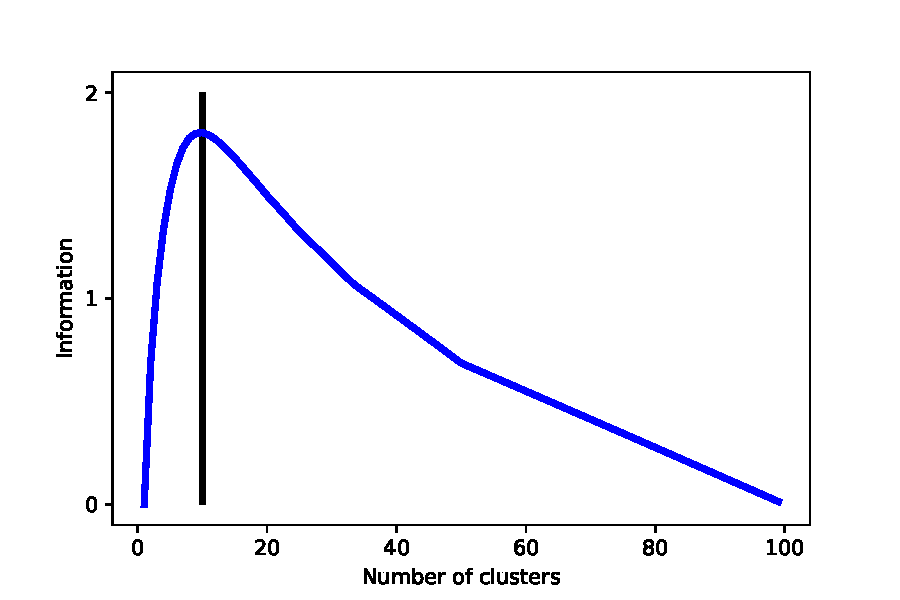
\includegraphics[width=7cm]{figures/info-100.pdf}
		\caption{Intrinsic information of a clustering of $n=100$ items into $k$ clusters, with respect to $k$.}
		\label{intrinsic_information}
	\end{center}
\end{figure}


\begin{figure}[h]
	\begin{center}
		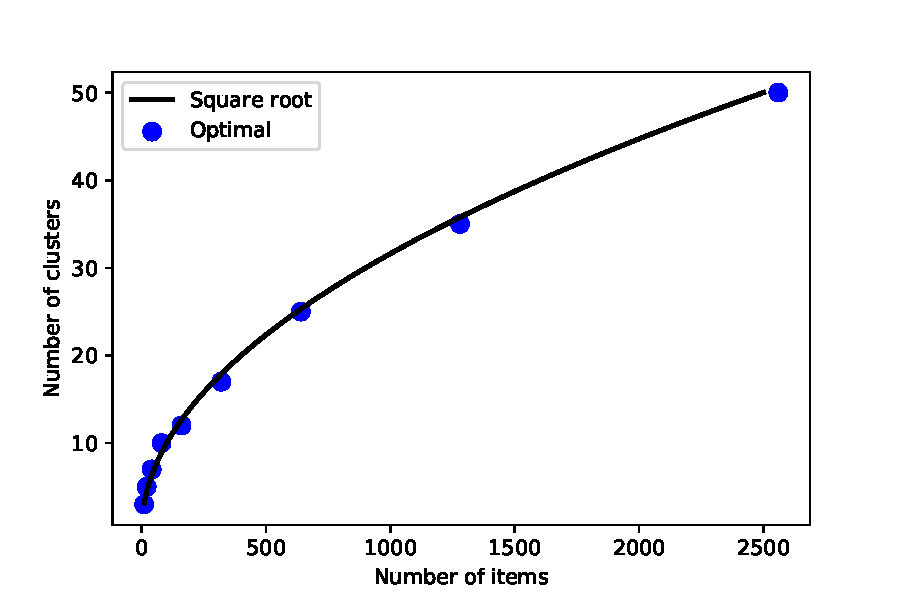
\includegraphics[width=7cm]{figures/sqrt.pdf}
		\caption{Optimal number of clusters with respect to  $n$.}
		\label{optimal_n_clusters}
	\end{center}
\end{figure}



\paragraph{Best cuts.}

%%TODO explain what is T

Find the cut that maximizes $h(A)$ for a given tree $T$. Find the best cuts, so that similarity $s(A,B)$ is maximum for two trees. Both benefit from the local change formulas \ref{eq:ami} -- \ref{eq:q}. The trivial cuts leading to $K=1$ or $K=n$ clusters are ruled out by the metric.

We justify the best cut property by the following experiments. 
Figure \ref{intrinsic_information} represents the type of experiment in where a set of data points are generated at random with total size $n=100$. Then we partition it in $K$ clusters from the range $\{1,\ldots,100\}$. We measure adjusted entropy for each set of labels and repeat the experiment 50 times with different randomisation and average results. Thereafter, it is clear that the peak of shared information to the number of clusters equals 10, a squared root of 100.   

The second experiment is conducted similarly but, instead, we consider datasets of different size $n$. We partition data points in clusters $K \in \{1,\ldots, n\}$ and calculate adjusted entropy for each set of labels. To identify an optimal number of clusters, we take the maximum index of all adjusted entropy scores. Finally, we can see in Figure \ref{optimal_n_clusters} that the optimal number of clusters and the squared root function have almost identical behaviour.

%%TODO Similarity

\paragraph{Similarity.} The similarity $s(A,B)$ between clusterings $A$ and $B$ is defined by $\ia(X,Y)$. This is the common information shared by $A$ and $B$ not due to noise. It is bounded by $\min(\log K, \log L)$. It can be negative if $A$ and $B$ share less information than noise. Observe that $s(A,A) = h(A)$. By Theorem \ref{th:ineq}, refining a clustering cannot increase  similarity: if $L > K > 1$ and each $B_j\in B$ is included in some $A_i\in A$, then  $s(A,B) < s(A,A)$. By Theorem \ref{th:ineq2}, two independent refinings of a clustering cannot increase  similarity: if $B'$ is another clustering with $L'$ clusters, such that $\max(L,L') > K > 1$, each $B_j\in B$ and each $B'_j\in B'$ are included in some $A_i\in A$, and $B_i \cap B'_{j} \in \{\emptyset, B_i, B'_j\}$, then  $s(B,B') < s(A,A)$. 

%Observe that we may have $s(B,B)\le s(A,A)$ or $s(B,B)> s(A,A)$. 

\section{Tree Mutual Information}
\label{algirithm}

\subsection{Algorithm}

\begin{algorithm}[h]
	\SetAlgoLined
	\KwIn{initial assignment $C_1$ and $C_2$, trees $T_1$ and $T_2$, set of nodes $V_1=\{root(T_1)\}$ and $V_2=\{root(T_2)\}$, maximum score $S^{max}=-1$}
	\KwOut{Score $S^{max}$}
	\tcp{returns a maximizing pair of nodes and a corresponding clustering}
	$S, T_1, T_2, C_1, C_2 = split(V_1, V_2, C_1, C_2)$\;
	\tcp{stop criteria}
	\If{$S<S^{max}$}{
		return $S^{max}$
	}
	\tcp{updates sets of nodes}
	$V_1 \leftarrow V_1  \backslash T_1$;  $V_1 \leftarrow V_1 \cup cut(T_1)$\;
	$V_2 \leftarrow V_2  \backslash T_2$;  $V_2 \leftarrow V_2 \cup cut(T_2)$\;
	return $TMI(C_1, C_2, V_1, V_2, S)$ 
	\caption{Tree Mutual Information(TMI).}
\end{algorithm}


\begin{algorithm}[h]
	\SetAlgoLined
	\KwIn{$C_1$, $C_2$, $V_1$, $V_2$}
	\KwOut{returns maximum value, a maximizing pair of nodes and a corresponding clustering $S^{max}, V_1^{max}, V_2^{max}, C_1^{max}, C_2^{max}$}
	\For{$node_1 \in V_1$} {
		$C_1 \leftarrow clustering(node_1)$ \;
		\For{$node_2 \in V_2$} 
		{$C_2 \leftarrow clustering(node_2)$ \;
			$S = similarity(C_1, C_2)$ \;
			\If{$S>S^{max}$}{
				$C_1^{max}, C_2^{max}, V_1^{max}, V_2^{max}$ = $C_1, C_2, V_1, V_2$ \;
			}    
		}
		\EndFor
	}
	\EndFor
	return $S^{max},C_1^{max}, C_2^{max}, V_1^{max}, V_2^{max}$ \;
	\caption{Split operation.}
\end{algorithm}

The algorithm takes as input a pair of dendrograms $D_1$ and $D_2$ with the same number of leaves $n$ and performs the following steps:

\begin{enumerate}
	\item Convert dendrograms $D_1$ and $D_2$ into a Newick format \cite{newick1990} - representation for trees $T_1$ and $T_2$ respectively.  
	\item Initialize 2 sets of nodes which we use to compare on every step: $V_1 = root(T_1)$ and $V_2 = root(T_2)$ for each of tree. Also initialize $S^{max}=-1$, $C_1^{max}$ and $C_2^{max}$ as trivial clustering.
	\item Consider the clustering $C_1$ induced by the top level of $T_1$ and the clustering $C_2$ induced by the top level of $T_2$ (top cuts). Compute $S = similarity(C_1, C_2)$, where $similarity(C_1, C_2)$ is one of our metrics: AMI defined by Equation \ref{eq:ami} or PAMI - Equation \ref{eq:pami}. If $S > S^{max}$ then update $C_1^{max}$ and $C_2^{max}$.
	\item Recursively repeat: whenever $S$ increases, change $C_1$ by going down in $T_1$ (lower cut). $C_1 = A \cup B$ where $A$ and $B$ are subclusters of $C_1$. Choose the best option from the set {$C_1$, $A$, $B$} which maximizes of $S$. Repeat the same for $C_2$: whenever $S$ increases, change $C_2$ by going down in $T_2$.
	\item Stop when $S$ cannot be increased. Return $S^{max}$.
\end{enumerate}

\subsection{Complexity}
\label{complexity}

%The most critical point is the complexity analysis. My suggestion is to impose a maximum limit on the number of clusters (in sqrt(n), say) to make the derivation cleaner. You can say that Property 4.1.1 suggests that this number will not be exceeded in practice.


To provide a closed form solution of algorithm complexity, we need to solve a discrete optimization problem that is not trivial. Hence, we are going to derive an approximated bound for the new metrics.  

Let's consider trees $T1$ and $T2$ with n-leaves. Let $A_i = \{A_{i1},\ldots,A_{ik_i}\}$ and $B_j = \{B_{j1},\ldots,B_{jl_j}\}$ be two partitions on trees' levels $i$, $j$ of some finite set $\{1,\ldots,n\}$ into $k_i$ and $l_j$ clusters, respectively. According to Property \ref{property_sqrt_n} the optimal numbers of clusters $k$ and $l$ are not exceeded by $\sqrt{n}$ in practice. We can get an approximation of complexity on the following parts:

\begin{enumerate}
\item Complexity of the metric: for AMI - $O(\max(k,l)n)$ and for PAMI - $O(kl)$.
\item Complexity of \textit{split} operation includes two nested loops of total size $\mid V_1 \mid \mid V_2 \mid$ which on each step calculate metric AMI or PAMI. Now using Property \ref{property_sqrt_n} we can roughly estimate a maximum number of nodes considered in \textit{split} operation. They are of size $\mid C_1 \mid < \sqrt{n}$ ,$\mid C_2 \mid < \sqrt{n}$ and that is why a combined complexity turns into $O(n)$. Therefore, depending on the metric, overall complexity of $split$ operation equals to $O(\max(k,l)n^2) \approx O(n^2))$ for AMI and $O(kln) \approx O(n)$ for PAMI.
\item The recursion $T(\sqrt{n}) = T(\sqrt{n}-1) + O(split)$ goes no further than one level deeper per step into trees structure. Finally, it results in the overall complexity: 

\begin{align}
\begin{split}
T(n) = O(n^{2.5})
\end{split}
\label{eq:complexity TAMI}
\end{align}	
for a Tree Mutual Information with AMI metric (TAMI)  

\begin{align}
\begin{split}
T(n) = O(n^{1.5})
\end{split}
\label{eq:complexity TPAMI}
\end{align}	
and for Tree Mutual Information with PAMI metric (TPAMI).   
\end{enumerate}

\subsection{Implementation details}
Obviously, the complexity of TAMI (\ref{eq:complexity TAMI}) is intractable for large graphs. Given this, we propose several options to reduce this complexity.
\paragraph{Sequential updates}
We can reduce AMI's complexity by one order $n$ making sequential updates on every step of $split$ algorithm instead of calculating it every time from scratch. Let's introduce sequential updates for the Mutual Information (MI) as well as for the Expected Mutual Information (EMI), which are defined in Formula \ref{eq:ami} as first and second term respectively. This is possible because we know precisely that we move maximum one level down into the tree hierarchy per step, local updates are sufficient. 

Variables $X$ and $Y$ are defined in the previous section and we introduce a new $Y^{'}$ random variable, which is obtained as an expanded version of $Y$ by going one level down in the tree. Let's assume that cluster $m$ was subdivided into $m^{'}$ and ${m+1}^{'}$ respectively. Consequently, in order to calculate probability for the new partitioning we should subtract $P(Y_m)log(P(Y_m))$ associated with cluster $m$ and add probability for new sub-clusters $m^{'}$ and ${m+1}^{'}$. It results in the following updated equations:

\begin{align*}
\begin{split}
H(Y^{'}) &= H(Y) - P(Y_m)log(P(Y_m)) + P(Y_m^{'})log(P(Y_m^{'})) + P(Y_{m+1}^{'})log(P(Y_{m+1}^{'})) 
\end{split}
\end{align*}

\begin{align*}
\begin{split}
H(X, Y^{'}) &=H(X,Y)-\sum_{i=1}^{|X|}P(X_i, Y_m)log(P(X_i, Y_m))  + \\
& + \sum_{i=1}^{|X|}P(X_i, Y_m^{'})log(P(X_i, Y_m^{'})) + \sum_{i=1}^{|X|}P(X_i, Y_{m+1}^{'})log(P(X_i, Y_{m+1}^{'})) \\ 
\end{split}
\end{align*}

\begin{align*}
\begin{split}
MI(X,Y^{'}) &= MI(X,Y) - P(Y_m)log(P(Y_m)) + P(Y_m^{'})log(P(Y_m^{'})) +  \\
&  + P(Y_{m+1}^{'})log(P(Y_{m+1}^{'})) + \sum_{i=1}^{|X|}P(X_i, Y_m)log(P(X_i, Y_m)) - \\
& - \sum_{i=1}^{|X|}P(X_i, Y_m^{'})log(P(X_i, Y_m^{'})) - \sum_{i=1}^{|X|}P(X_i, Y_{m+1}^{'})log(P(X_i, Y_{m+1}^{'})) 
\end{split}
\end{align*}


Similarly, for $EMI$: $Y'=[Y_1, \dots Y_m^{'}, Y_{m+1}^{'}, \dots Y_{l}]$. In order to have a new score $EMI(X,Y^{'})$, we need to update following components: $b=[b_1, \dots b_m, \dots b_l]$ to $b=[b_1 \dots b_m^{'}, b_{m+1}^{'}, \dots b_l]$. Let's define this new notation:

\begin{equation}
\begin{split}
f(b_m) = \sum_{i=1}^{k}\sum_{c_{m}=(a_i+b_m-n)^+}^{\min(a_i, b_m)} 
\frac{a_i!b_m!(n-a_i)!(n-b_m)!}{n!c_{m}!(a_i-c_{m})!(b_m-c_{m})!(n-a_i-b_m+c_{m})!}\frac{c_{m}}{n}\log \left( \frac{ c_{m}}{n}\right)
\end{split}
\end{equation}

Then $EMI(C_1, C_2^{'})$ can be calculated as:

\begin{equation}
EMI(C_1, C_2^{'}) = EMI(C_1, C_2) - f(b_m) + f(b_m^{'}) + f(b_{m+1}^{'})
\end{equation}

By the same logic, we can obtain updates for $a$.

\paragraph{Cashing}
\label{cashing}
Complexity can similarly be reduced by the use of cashing. Because of the construction of Equation \ref{eq:ami} this can be efficiently performed. So as to calculate TAMI we employ Formula \ref{eq:ami}. The time complexity of this formula is dominated by the second term equal to $O(\max(k,l)n)$. We can rewrite Equation \ref{eq:ami} $$\sum_{i=1}^{k}\sum_{i=j}^{l}f(a_i,b_j,n)$$ as stated in Equation \ref{eq:precomputed_ami}. It only depends on parameters $a_i$, $b_j$ and $n$. As a result, we discard term $n$ in summation which reduces the overall complexity to $O(kl)$. This trick significantly speedups computation by summing up over cashed terms during execution.

\begin{align}\label{eq:precomputed_ami}
\begin{split}
f(a_i,b_j,n) =\sum_{c = (a_i+b_j - n)^+}^{\min(a_i, b_j)} \frac{a_i!b_j!(n-a_i)!(n-b_j)!}{n!c!(a_i-c)!(b_j-c)!(n-a_i-b_j+c)!}\frac {c}n \log \frac {c}n.
\end{split}
\end{align}